
\slidesectionwithgraphic{Discussion}{images/evocells-demo-compressed.jpg}

\begin{frame}{Discussion}
	\begin{columns}[T,onlytextwidth]
		\begin{column}{0.5\textwidth}
			\textbf{Insights}
			\begin{itemize}
				\item Aim at the most specific category
				\item All visualization techniques covered by this taxonomy use an underlying treemap layout
				\item Only a systematic top-down or bottom-up approach adhering to the containment metaphor results in a treemap
			\end{itemize}
			\textbf{Limitations}
			\begin{itemize}
				\item Taxonomy does not cover mixed-use of treemaps and basic forms of subdivision
				\item Taxonomy does not cover all tree visualization techniques
				\item Conceptual border between mapped trees and general tree and hierarchy visualization techniques to be determined
			\end{itemize}
		\end{column}
		\begin{column}{0.5\textwidth}
			\begin{figure}
				\centering
				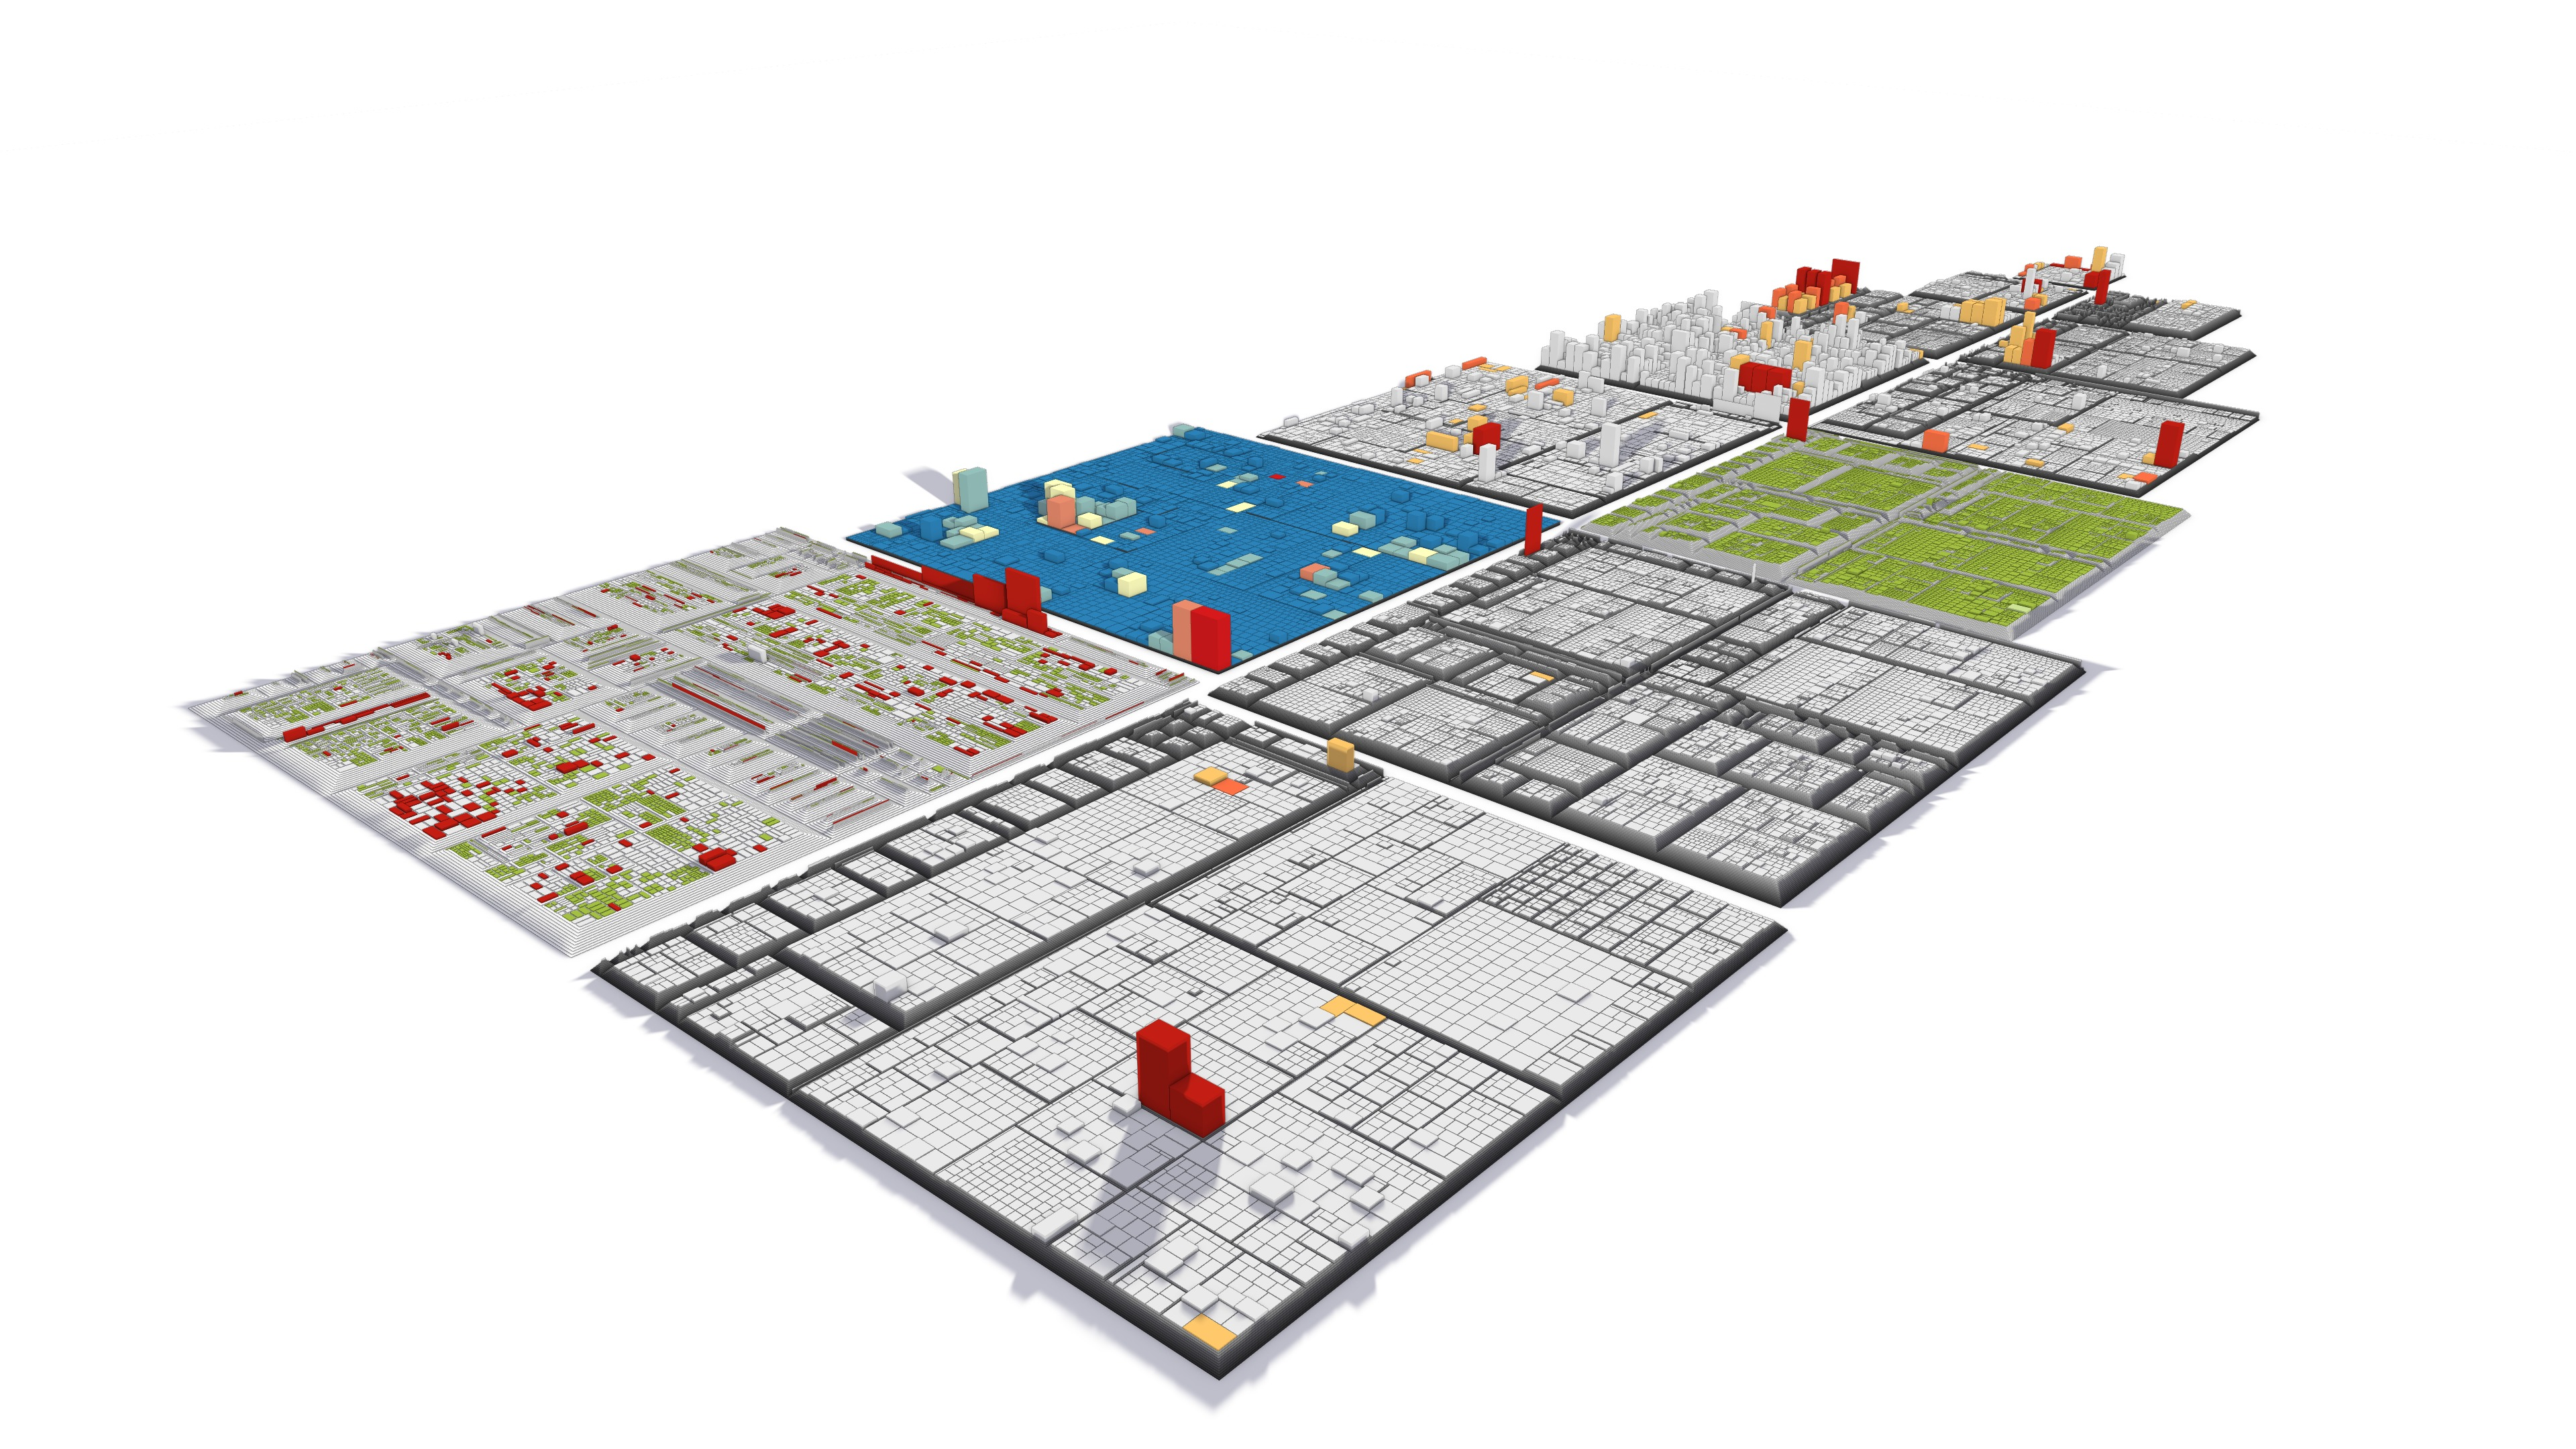
\includegraphics[width=1.0\linewidth]{images/treemaplandscape.jpg}
				\caption{Adjacent placement of multiple treemap visualizations.}
			\end{figure}
		\end{column}
	\end{columns}
\end{frame}

\begin{frame}[c]{Comparison to General Hierarchy Visualization Techniques}
	\begin{figure}
		\centering
		\footnotesize
		\begin{tikzpicture}[every node/.style={inner sep=0,outer sep=0},node distance=0pt]
		\node[] (sot-1) {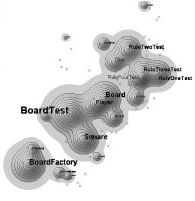
\includegraphics[width=\exampleslargewidth]{figures/thematicsoftwaremaps.png}};
		\node[below=5pt of sot-1,text width=0.7\exampleslargewidth,align=center] (sot-1-label) { Thematic Software Maps };
		\node[right=10pt of sot-1.north east,anchor=north west] (sot-2) {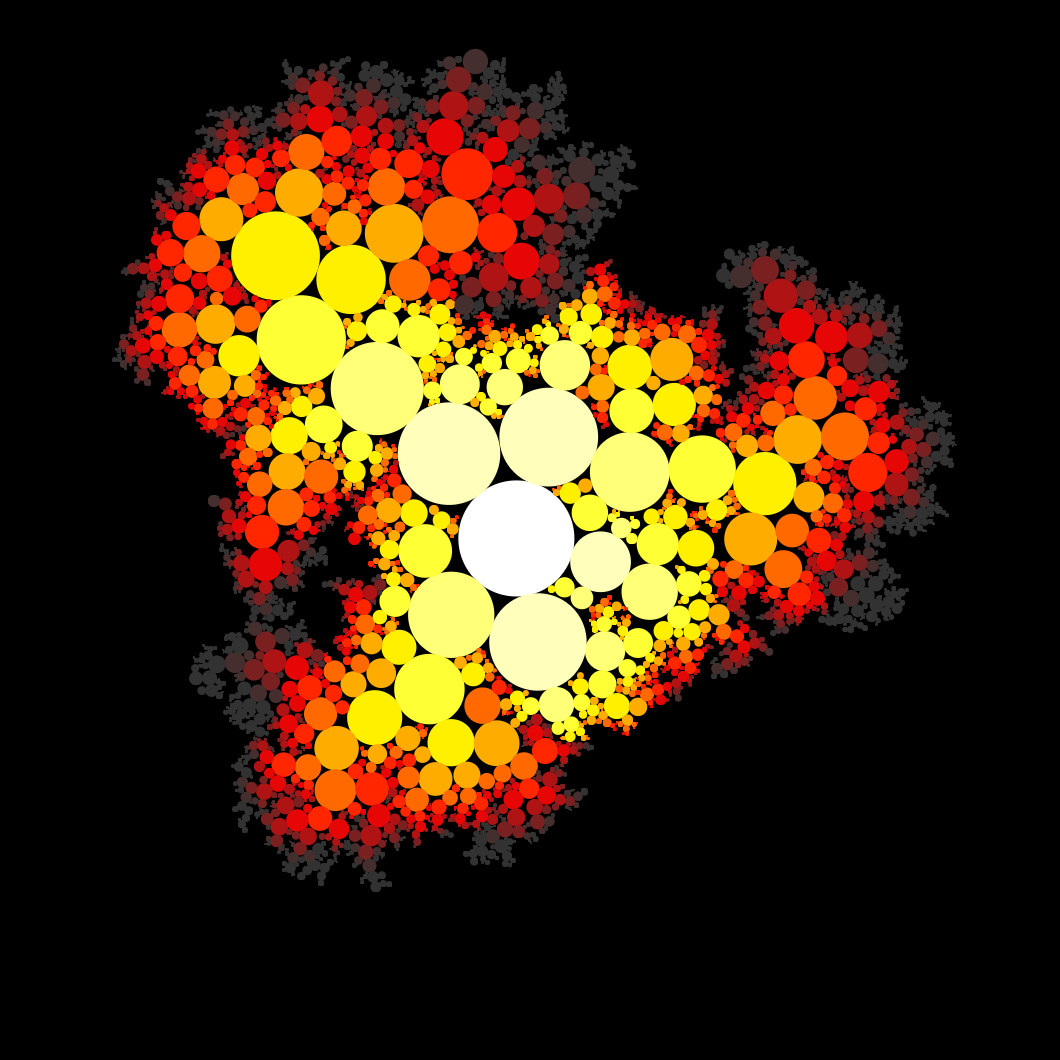
\includegraphics[width=\examplesdefaultwidth]{figures/bubblehierarchy.png}};
		\node[below=5pt of sot-2,text width=\examplesdefaultwidth,align=center] (sot-2-label) { Bubble Hierarchies };
		\node[right=10pt of sot-2] (sot-3) {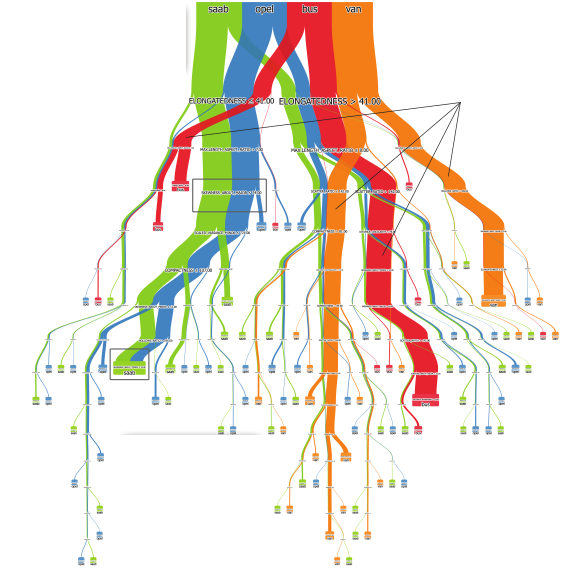
\includegraphics[width=\examplesdefaultwidth]{figures/baobabview.png}};
		\node[below=5pt of sot-3,text width=\examplesdefaultwidth,align=center] (sot-3-label) { BaobabView };
		\node[right=10pt of sot-1.south east,anchor=south west] (sot-4) {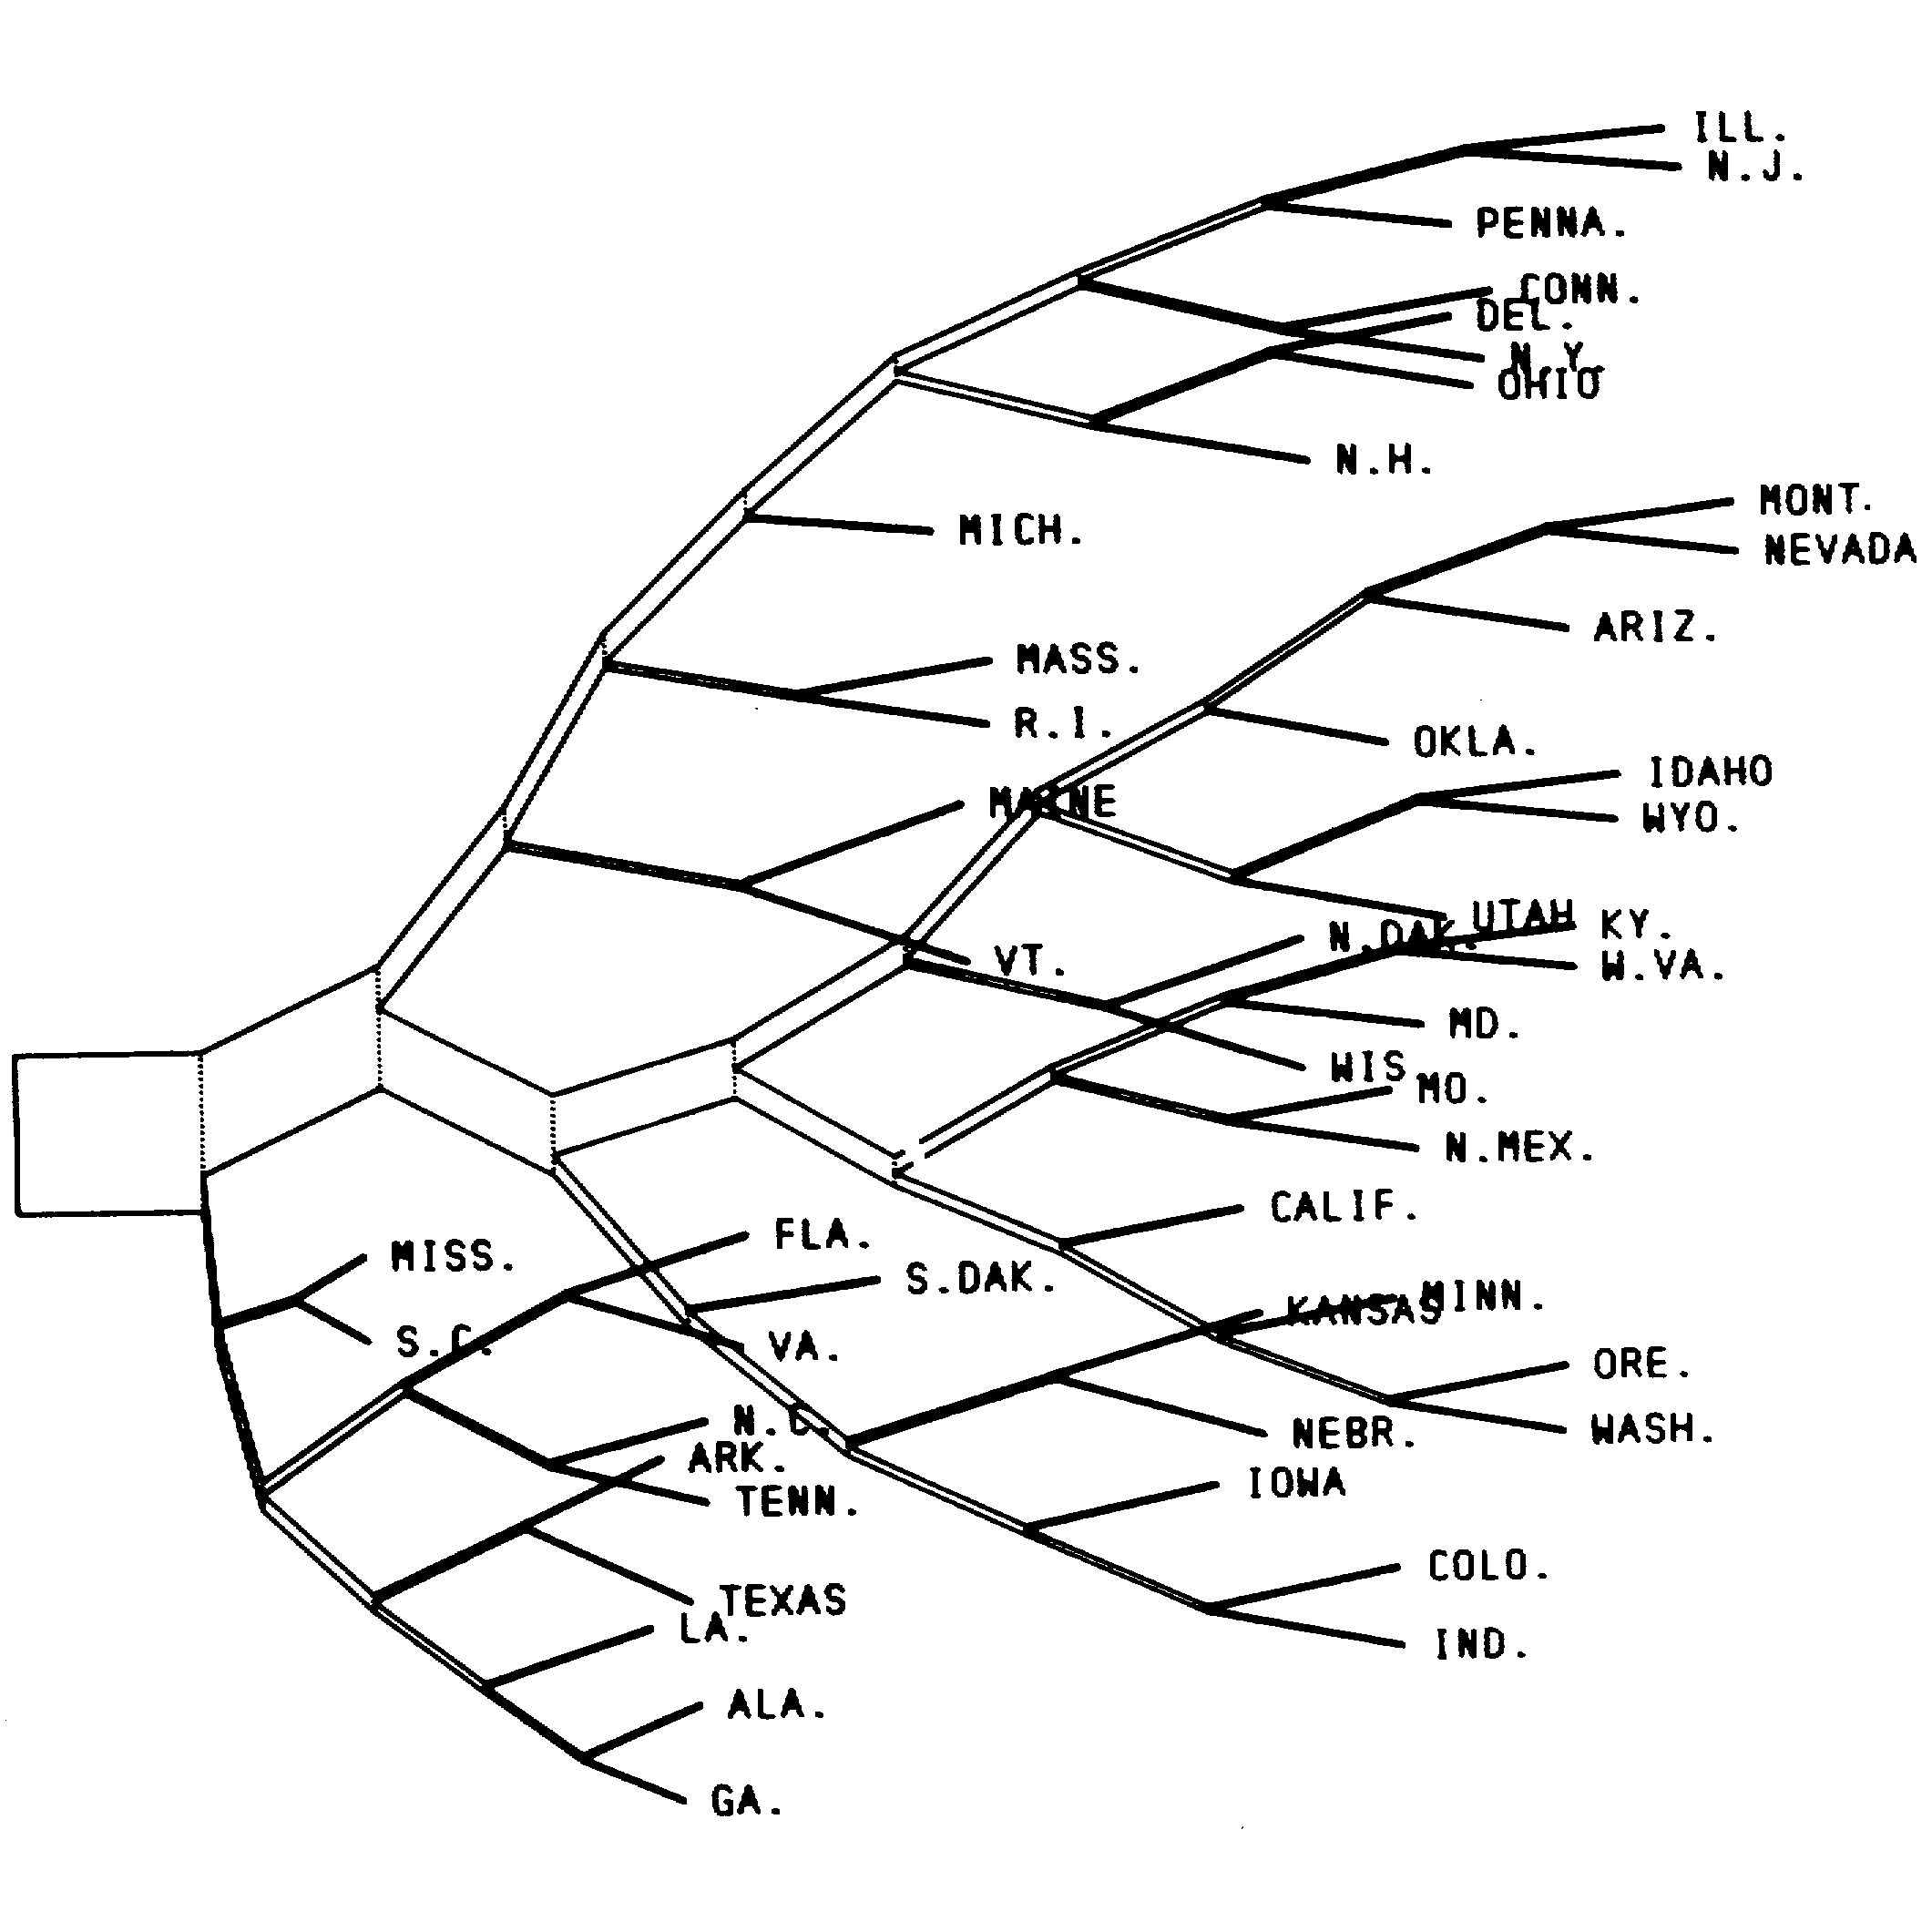
\includegraphics[width=\examplesdefaultwidth]{figures/tree.png}};
		\node[below=5pt of sot-4,text width=\examplesdefaultwidth,align=center] (sot-4-label) { Tree of Percentage };
		\node[right=10pt of sot-4] (sot-5) {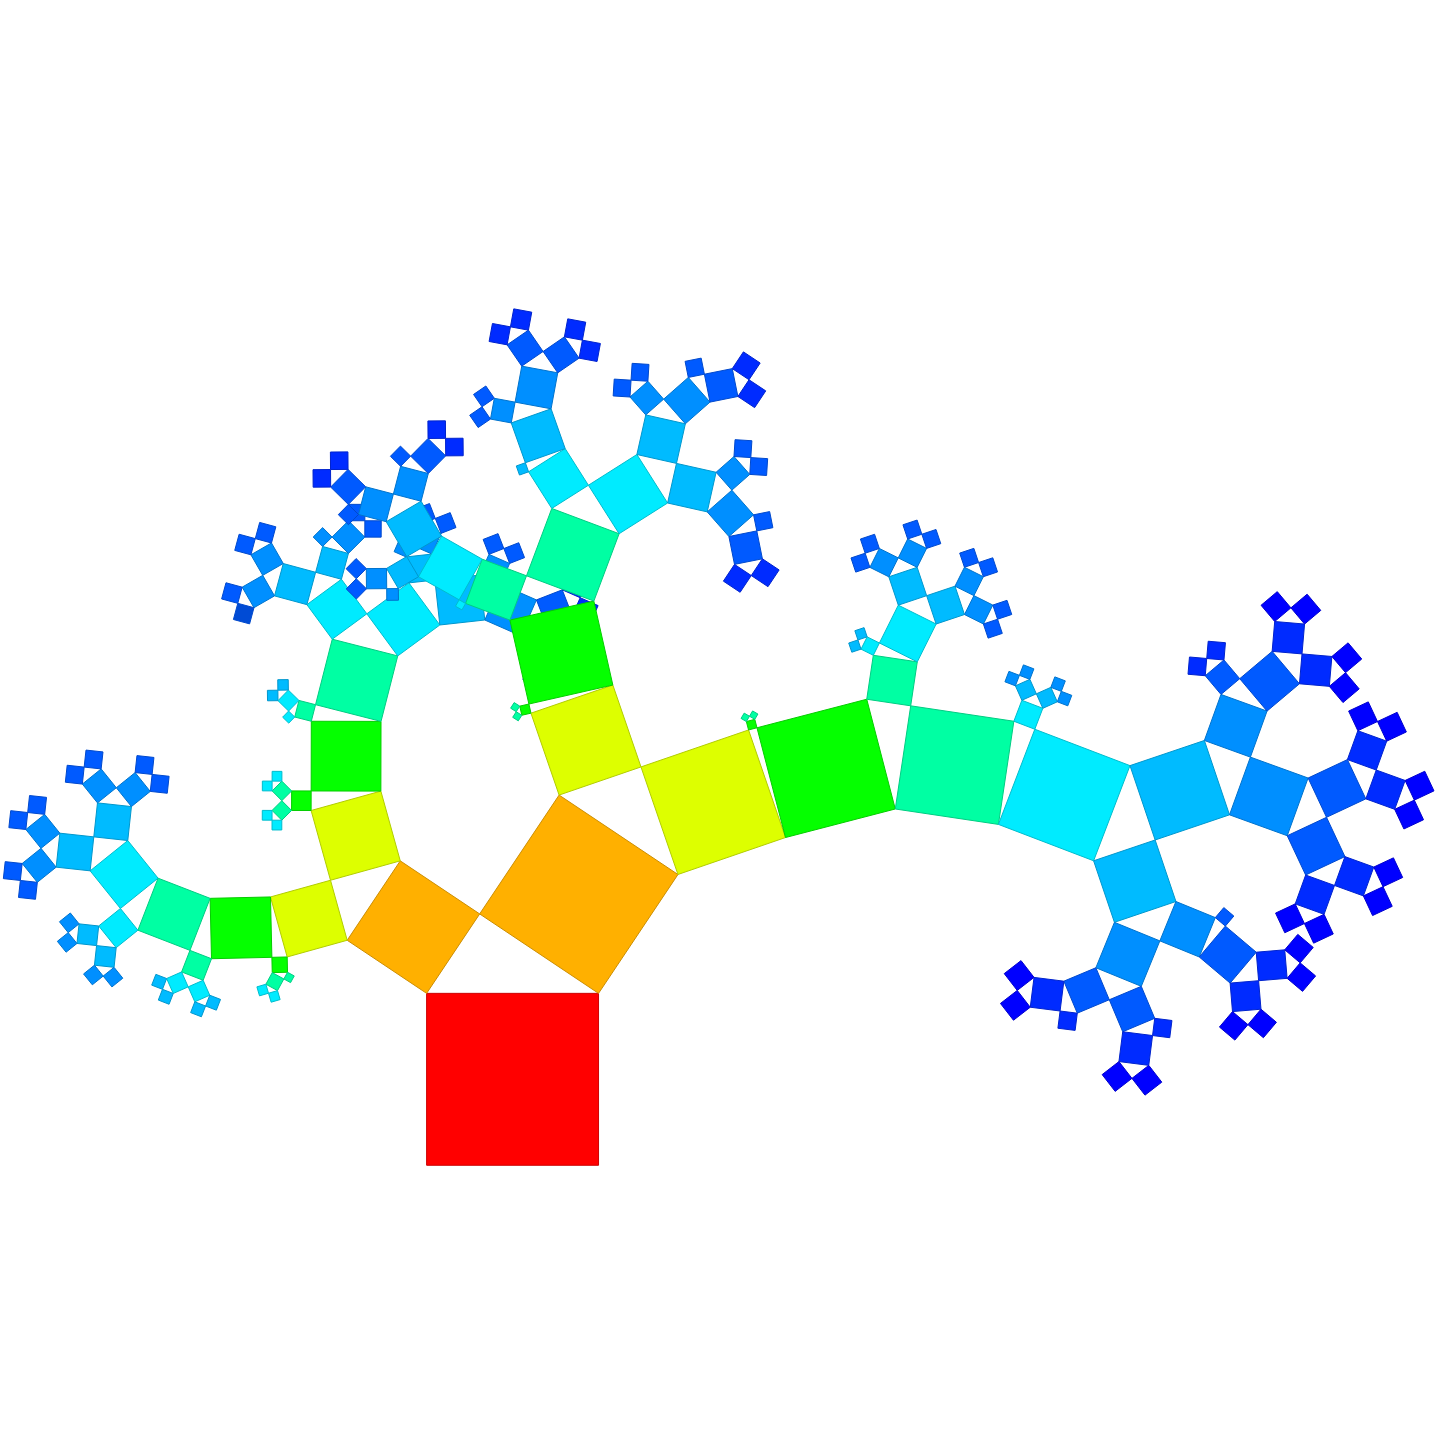
\includegraphics[width=\examplesdefaultwidth]{figures/pythagorastree.png}};
		\node[below=5pt of sot-5,text width=\examplesdefaultwidth,align=center] (sot-5-label) { Pythagoras Tree };
		\node[above=5pt of sot-2.north west,xshift=-5pt] (Th) { \Th };
		\draw[thin,black,shorten >= 10pt] (Th-|sot-1.west) -- (Th);
		\draw[thin,black,shorten <= 10pt] (Th) -- (Th-|sot-3.east);
		\end{tikzpicture}
		\caption{Examples of visualization techniques that does not relate to any proposed class and are therefore associated with \Th{}. Image courtesy from left to right and top to bottom: \cite{kuhn2010-thematic}, \cite{hlawatsch2014-bubblehierarchies}, \cite{andrews1998-slices}, \cite{elzen2011-baobabtrees}, \cite{kleiner1981-trees}, and \cite{beck2014-pythagorastrees}.}
	\end{figure}
\end{frame}
